\documentclass{beamer}
%\usepackage[margin=1in]{geometry}
\usepackage{amsmath}
\usepackage{amsfonts}
\usepackage{esint}
\usepackage{ mathrsfs }
\usepackage{graphicx}
\graphicspath{{chapter_8_figures/}}
\usetheme{Berlin}
\numberwithin{equation}{section}
\title{Alternating Current}
\date{Spring 2017}
\author{Alex Coy \and Sam Ehrenstein \and Noah Friedlander \and Eshan Tewari}
\newcommand{\Lapl}{\mathscr{L}}
\begin{document}
\maketitle

\begin{frame}
\frametitle{The Series RLC Circuit}
\begin{columns}
\column{0.55\textwidth}
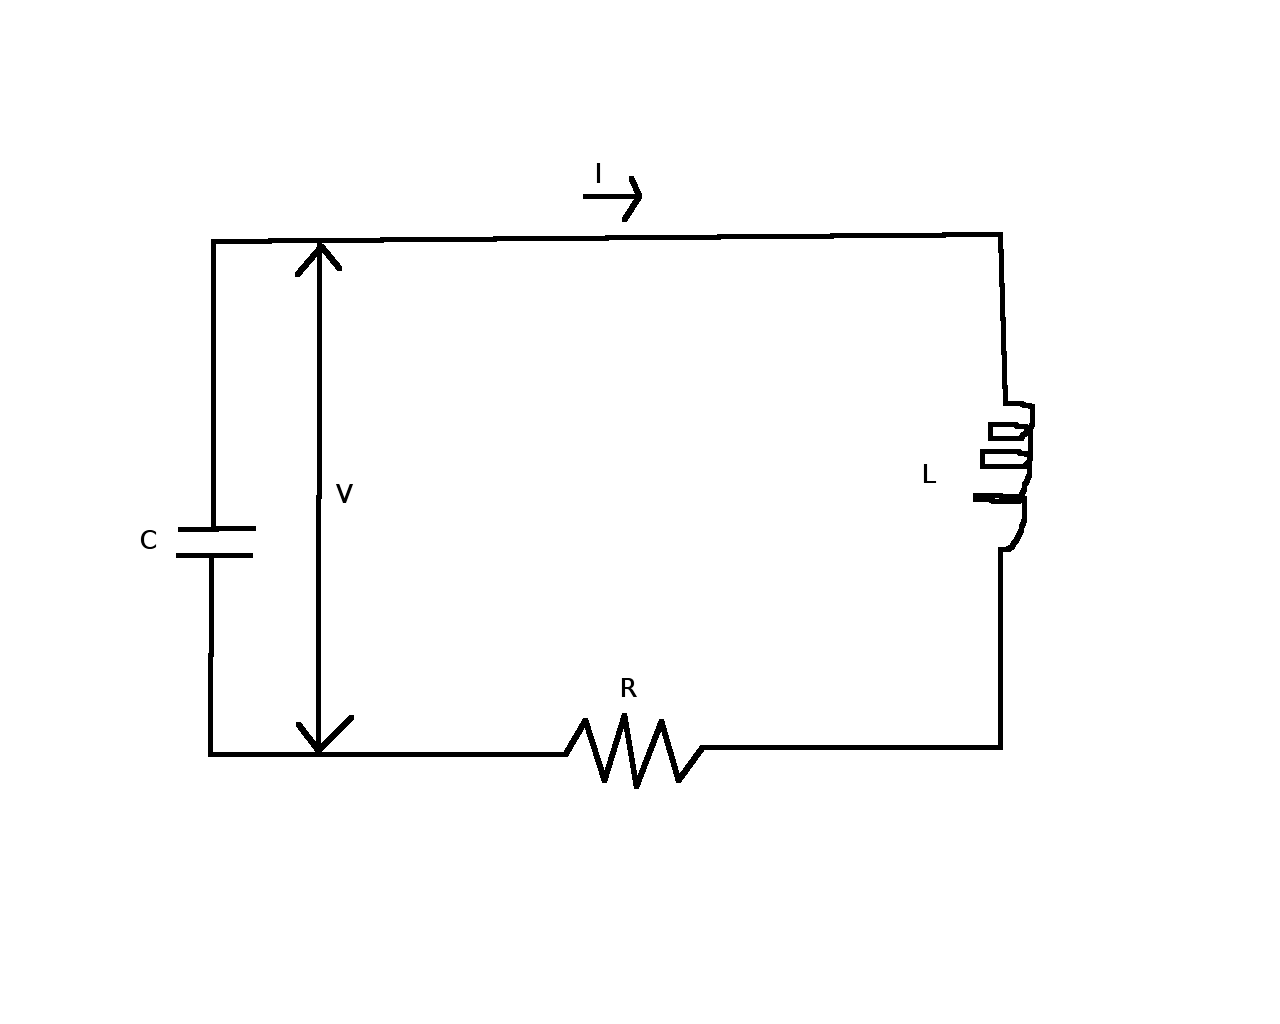
\includegraphics[width=\textwidth]{series_rlc}
\column{0.5\textwidth}
Governing equations:
\begin{itemize}
\item
$I=-\frac{dQ}{dt}$
\item
$Q=CV$
\item
$V=L\frac{dI}{dt}+RI$
\end{itemize}

Write Q and I in terms of V to get
\[\frac{d^2V}{dt^2}+\bigg(\frac{R}{L}\bigg)\frac{dV}{dt}+\bigg(\frac{1}{LC}\bigg)V=0\]
\end{columns}
\end{frame}


\begin{frame}
\frametitle{That's a Spring}
Multiply through by L to get
\[L\frac{d^2V}{dt^2}+R\frac{dV}{dt}+\frac{1}{C}V=0 \iff m\frac{d^2x}{dt^2} + b\frac{dx}{dt}+kx=0\]

\begin{itemize}
\item
L has ``intertia" that resists change
\item
The resisitor provides a drag force
\item
The capacitor provides a restoring force
\end{itemize}
\end{frame}

\begin{frame}
\frametitle{$\zeta(r)$ as an Euler Product}
\[\zeta(r) = \sum_{n} \frac{1}{n^r}=\prod_p \frac{1}{1-p^{-r}}\]
\[\text{where p is a prime number}\]
Sit back and enjoy the justification of this. It'll be on Edline this evening.
\end{frame}


\end{document}